\documentclass[11pt]{article}
\usepackage{epsfig}
\usepackage{epstopdf}
\usepackage[top=1in,right=1in,left=1in,bottom=1in]{geometry}
\pagestyle{empty}
%\usepackage{fullpage}
%\topmargin 0.0in
%\headheight 0.0in
%\pagestyle{empty}

\begin{document}




\title{Explanation of low Hurst exponent for Riemann zeta zeros}


\author{O. Shanker \thanks{O. Shanker is with Hewlett-Packard (oshanker@gmail.com)}
}

\date{}

\maketitle
\thispagestyle{empty}

\begin{abstract}
We discuss a possible explanation for the low Hurst exponent
extracted from a rescaled range analysis
of the large height Riemann zeta function zeros.
\end{abstract}

\markboth{O. SHANKER}{Generalised Zeta Functions}

Physicists have studied the zeros of the Riemann zeta function
because of its  relation
to the spectra of random matrix theories (RMT)
\cite{Wigner(1967),Gaudin and Mehta (1960),Gaudin(1961),Dyson(1962)}
and the spectra of classically chaotic quantum
systems~\cite{Berry(1985),Berry(1986),Berry(1987),Berry(1988)}.
A rescaled range analysis
of the large height Riemann zeta zeros leads to
a very low Hurst exponent ($\sim 0.1$)
over several orders of magnitude variation
(from $10^{7}$ to $10^{22}$) in the heights of the zeros~\cite{os6}.
So far there has been no explanation for this behaviour.
One possible explanation is that the zeros
represent a long range anti-correlation. However, one has to
be careful in coming to that conclusion, since such a large anti-correlation
is rather special~\cite{Govind}. In this work we
argue that the low Hurst exponent is not due to an anti-correlation,
but can be explained by superposing a random Gaussian correction
term to Riemann's approximation
for the variation of the number of zeros with height.

We first briefly set up the notation.
The Riemann Zeta function is defined for $\mathrm{Re} (s) > 1$ by
\begin{equation}
\zeta ( s ) \, = \, \sum^{\infty}_{n = 1} \; n^{-s} \, = \, \prod_{p} \;
\left( 1 - p^{-s} \right)^{-1}.
\label{eqRie}
\end{equation}
$\zeta ( s )$ has a  continuation
to the complex plane and satisfies a functional equation
\begin{equation}
\xi(s):= \pi^{-s/2} \, \Gamma (s/2) \, \zeta ( s ) \, = \, \xi ( 1 - s );
\label{eq:func}
\end{equation}
$\xi(s)$ is entire except for simple poles at $s = 0$ and $1$.  We
write the zeroes of $\xi(s)$ as $1/2 + i \gamma$.
The Riemann Hypothesis~\cite{Riemann(1858),Riemann(1892),Titchmarsh(1986),Edwards(1974)}
asserts that $\gamma$ is real for the non-trivial zeroes.
We order the $\gamma$s in increasing order, with
\begin{equation}
\ldots \ldots \gamma_{-1} \, < \, 0 \, < \,
\gamma_1 \, \leq \, \gamma_2 \ldots.
\end{equation}
Then $\gamma_j \, = \, - \gamma_{-j}$ for $j = 1, 2, \ldots,$
and    $\gamma_1$, $\gamma_2$, $\ldots$  are roughly
$14.1347$, $21.0220$, $\ldots$.
The Hurst exponent is extracted by applying rescaled range analysis
to the distribution of the spacings~\cite{os6}
$\delta_j\, = \, \gamma_{j + 1} \, - \, \gamma_j$.

From Riemann's time it is known that the mean number of
zeros with height less than $\gamma$ (the smoothed Riemann zeta staircase)
is approximately~\cite{Edwards(1974),Berry(1986)}
\begin{equation}
<\mathcal{N_R} (\gamma)> = (\gamma/2\pi)(ln(\gamma/2\pi)-1)+\frac{7}{8}.
\label{eq:Rnumber}
\end{equation}
Thus, the mean spacing of the zeros at height $\gamma$ is
$2\pi(\ln (\gamma/2\pi))^{-1}$. Eqn.~\ref{eq:Rnumber} can be
inverted to give an
approximation $\gamma_{a,i}$ for the $i^{th}$ zero of the
Riemann zeta function, if we set $<\mathcal{N_R} >=i$.
Let us write the $i^{th}$ zero $\gamma_{i}$ as
\begin{equation}
\gamma_{i} = \gamma_{a,i}+X_{i},
\label{eq:zero}
\end{equation}
where $X_{i}$ is a correction term. We show that the observed
behaviour of the rescaled range analysis is reproduced even if
there is no anti-correlation between the Riemann zeta zeros,
all that is needed is to assume that the correction term $X_{i}$
is distributed normally. With this assumption, Table~\ref{tab:table1}
shows the Hurst exponent extracted from the Riemann zeta zeros,
and for comparision the Hurst exponent for the sequence
given by Eqn.~\ref{eq:zero} with $X_{i}$ distributed normally.
We ran the analysis using
two different seed values for the random number generator.
The standard deviation of the
normal distribution was taken to be $0.25$ .
We see from the table that Eqn.~\ref{eq:zero}
reproduces the observed behaviour of the Riemann zeros fairly
well. It is also not too sensitive to the assumed seed value used
to generate the Gaussian term $X_{i}$ in Eqn.~\ref{eq:zero}.
Finally, it reproduces the observed low Hurst exponent for the
large height zeros, since for these zeros the first term
in Eqn.~\ref{eq:zero} becomes essentially linear, and the
Hurst exponent is then determined by the normal term, independent of the
height. Thus, it appears that the observed low value for the large
height Riemann zeta zeros is not due to an anti-correlation, but
instead it is due to the fact that for these zeros the
dependence on height is essentially linear, with a normal correction
term superposed on the linear variation.

Figure~\ref{fig_1} shows the
rescaled range analysis for
the zeros  in the range $100000 \ldots 110000$.
The horizontal
axis is the log of the bin size used for the rescaled range analysis,
and the
vertical axis is the log of the mean rescaled
range for the given values of bin size. The low slope
at the low values of the bin size is due to the
$X_{i}$ term in Eqn.~\ref{eq:zero}, and the increase in
slope at higher bin sizes is due to the
$\gamma_{a,i}$ term in Eqn.~\ref{eq:zero}. Eqn.~\ref{eq:zero}
gives a fairly good representation of the rescaled
range behaviour of the actual Riemann zeta zeros.

\begin{table}
\caption{Hurst Exponent for Riemann zeroes
and for the values from Eqn.~\ref{eq:zero} with two
different seed values for the random number generator.
The sample size is $10000$ and the standard deviation
for $X_{i}$ in Eqn.~\ref{eq:zero} is 0.25}
\begin{center} \footnotesize
\begin{tabular}{|c|c|c|c|} \hline
Range of zeroes&Riemann &Eqn.~\ref{eq:zero} &Eqn.~\ref{eq:zero} \\
 & zeros & seed A & seed B \\
\hline
$10^{4} < j \leq 2*10^{4}$ & 0.51 & 0.51& 0.51\\
$10^{5} < j \leq 10^{5} + 10^{4}$ & 0.21 & 0.21& 0.20\\
$10^{6} < j \leq 10^{6} + 10^{4}$ & 0.10 & 0.13&0.11\\
$10^{12} < j \leq 10^{12} + 10^{4}$ & 0.12 & 0.12&0.11\\
$10^{22} < j \leq 10^{22} + 10^{4}$ & 0.12 & 0.12&0.11\\
\hline
\end{tabular}
\end{center}
\label{tab:table1}
\end{table}


\begin{figure}
\vspace {5pt}
\centering
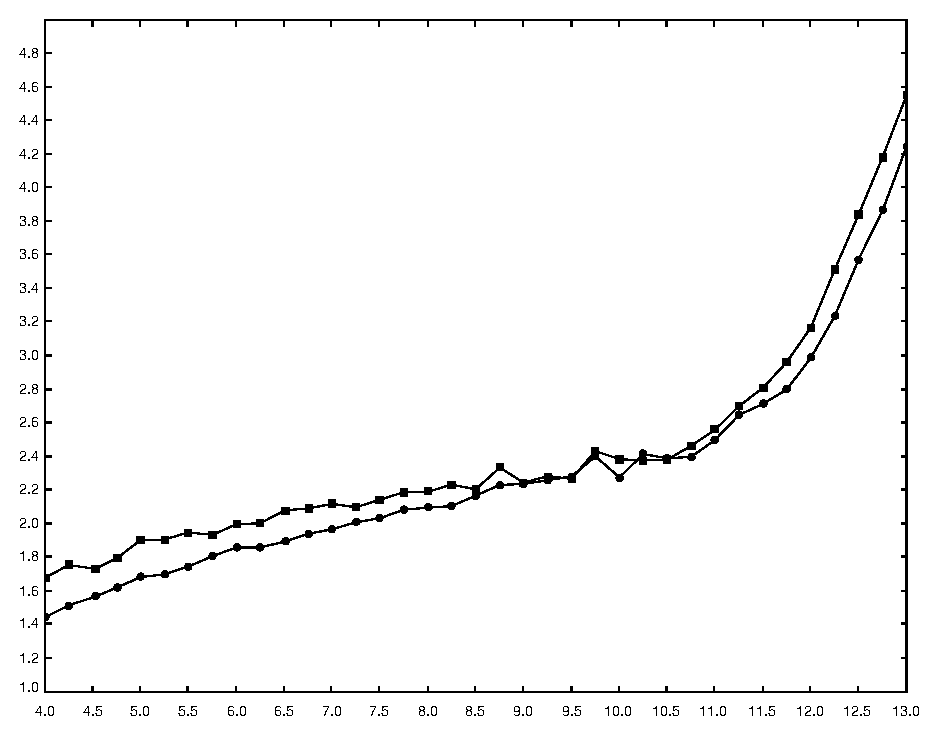
\includegraphics[width=5in,height=5in]{fig_1}
\caption{  Rescaled range analysis for
the zeros  in the range $100000 \ldots 110000$.
The y axis is the log of
the rescaled range
and the x axis is the log of the bin size.
Squares represent the values for the Riemann zeros
and circles represent the values for the sequence in
Eqn.~\ref{eq:zero}}.
\label{fig_1}
\end{figure}

In conclusion, we have presented evidence that the remarkable
behaviour of the Riemann zeta zeros under rescaled range analysis
can be explained by Riemann's approximation
for the variation of the number of zeros with height coupled with a
random Gaussian correction term.





\begin{footnotesize}
\begin{thebibliography}{10}

\bibitem {Wigner(1967)} E. Wigner, ``Random Matrices in Physics,'' {\it Siam
Review}, {\bf 9}, 1-23, (1967).

\bibitem{Gaudin and Mehta (1960)} M. Gaudin, M. Mehta, ``On the Density of Eigenvalues of a
Random Matrix,'' {\it Nucl. Phys.}, {\bf 18}, 420-427, (1960).

\bibitem{Gaudin(1961)} M. Gaudin, ``Sur la loi Limite de L'espacement de Valuers
Propres D'une Matrics Aleatiore,'' {\it Nucl. Phys.}, {\bf 25}, 447-458,
(1961).

\bibitem{Dyson(1962)} F. Dyson, ``Statistical Theory of Energy Levels III,''
{\it J. Math. Phys.}, {\bf 3}, 166-175, (1962).

\bibitem{Berry(1985)} M. V. Berry,
``Semiclassical theory of spectral rigidity,''
{\it Proc. R. Soc.}, {\bf A 400 }, 229-251, (1985).


\bibitem{Berry(1986)} M. V. Berry,
``Riemann's zeta function: a model for quantum chaos?,''
{\it Quantum chaos and statistical nuclear physics
(Springer Lecture Notes in Physics)}, {\bf 263 }, 1-17, (1986).


\bibitem{Berry(1987)} M. V. Berry, ``Quantum Chaology,''
{\it Proc. R. Soc. }, {\bf A 413 }, 183-198, (1987).


\bibitem{Berry(1988)} M. V. Berry, `Number variance of the Riemann zeros`,''
{\it NonLinearity }, {\bf 1 },399-407 , (1988).


\bibitem{os6} O. Shanker,
Generalised Zeta Functions and Self-Similarity of Zero Distributions,
{\it J.  Phys. A} {\bf39}(2006), 13983-13997.

\bibitem{Govind}
Govind Rangarajan and Mingzhou Ding,
\newblock ``An Integrated Approach to the Assessment of Long Range
Correlation in Time Series Data'',
{\it Phys. Rev.}, {\bf E61}, 4991-5001, (2000).

\bibitem {Riemann(1858)} B. Riemann, ``\"{U}ber die Anzahl der Primzahlen uter

Einer Gegebenen Gr\"{o}be,'' {\it Montasb. der Berliner Akad.}, (1858),
671-680.

\bibitem {Riemann(1892)} B. Riemann, ``Gesammelte Werke'', Teubner, Leipzig, (1892).

\bibitem {Titchmarsh(1986)} E. Titchmarsh, ``The Theory of the Riemann Zeta
Function,'' Oxford University Press, Second Edition, (1986).

\bibitem {Edwards(1974)} H. M. Edwards, ``Riemann's Zeta Function,''
Academic Press,  (1974).

\end{thebibliography}
\end{footnotesize}

\end{document}

